%!TEX root = ../dokumentation.tex

\chapter{Inbetriebnahme}

%TODO Bild von kompletten Aufbau
Der Bildschirm muss an den HDMI-Ausgang des Raspberry Pi angeschlossen werden (weißes Kabel). Anschließend wird das Flachbandkabel der Verteiler-Platine befestigt. Die Seite mit der roten Leitung muss bündig auf die Pins gesteckt werden, auf der anderen Seite bleiben einige Pins unbenutzt. Anschließend kann die Stromversorgung über das Mikro-USB-Kabel hergestellt werden (schwarzes Kabel). Der Computer startet daraufhin automatisch.\\
\begin{figure}[H]
	\centering
	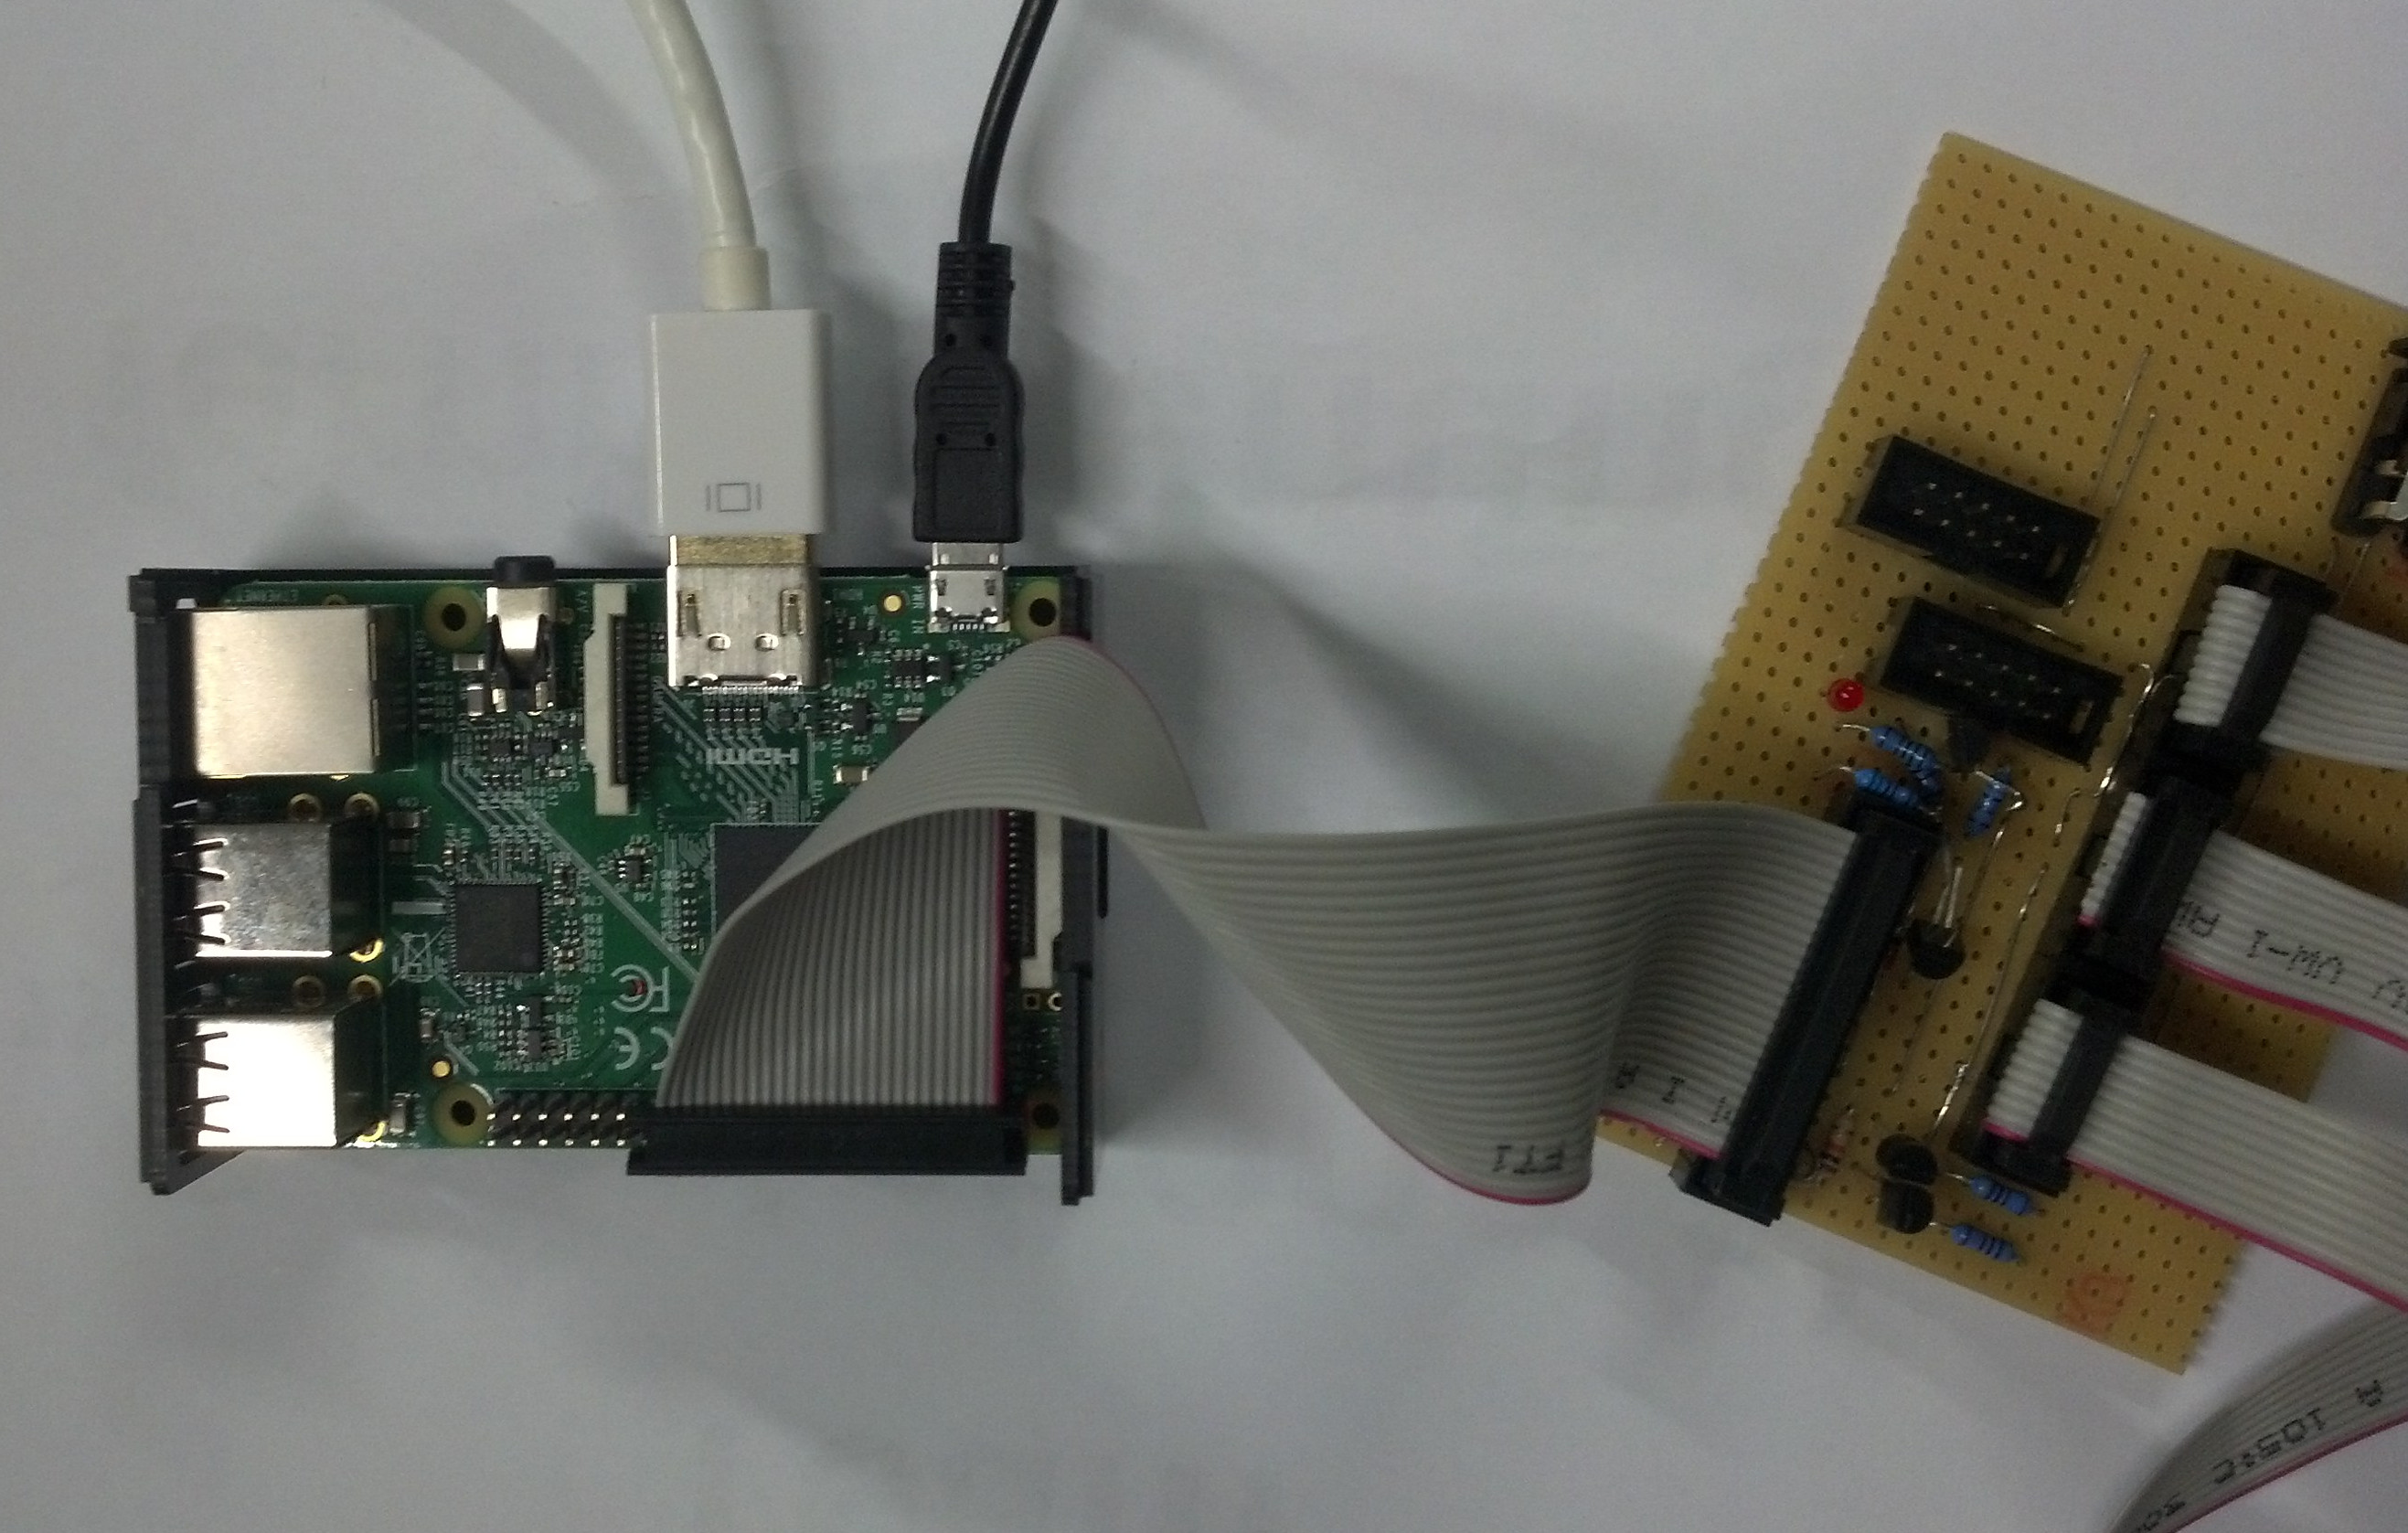
\includegraphics[width=(\textwidth), angle=0]{fotos/rasp.jpg}
	\caption{Verkabelung des Raspberry Pi} \label{p:1}
\end{figure}
Die drei Sensorplatinen werden auf den oberen drei kleinen Steckplätzen der Verteiler-Platine befestigt, die Reihenfolge spielt dabei keine Rolle. Die übrigen zwei Steckplätze wurden verwendet, um die Mikrocontroller zu programmieren und werden nicht mehr benötigt. Anschließend wird die Stromversorgung eingesteckt, woraufhin die Platinen einige Signale über die LEDs ausgeben. Die kleinen Sensorplatinen wechseln in den Wartezustand, bis eine Verbindung mit ihnen aufgebaut wird (rote LED pulsiert). Die große Sensorplatine führt automatisch Distanzmessungen aus und zeigt die Ergebnisse auf der 7-Segment-Anzeige an. Sobald eine Verbindung (z.B. über die GUI) aufgebaut wurde, stoppen die automatischen Messungen, damit es zu keinen Signalüberlagerungen während der Positionsbestimmung kommt. Die Mikrocontroller können über den Reset-Knopf in ihren Ausgangszustand zurück gebracht werden.\\
\begin{figure}[H]
	\centering
	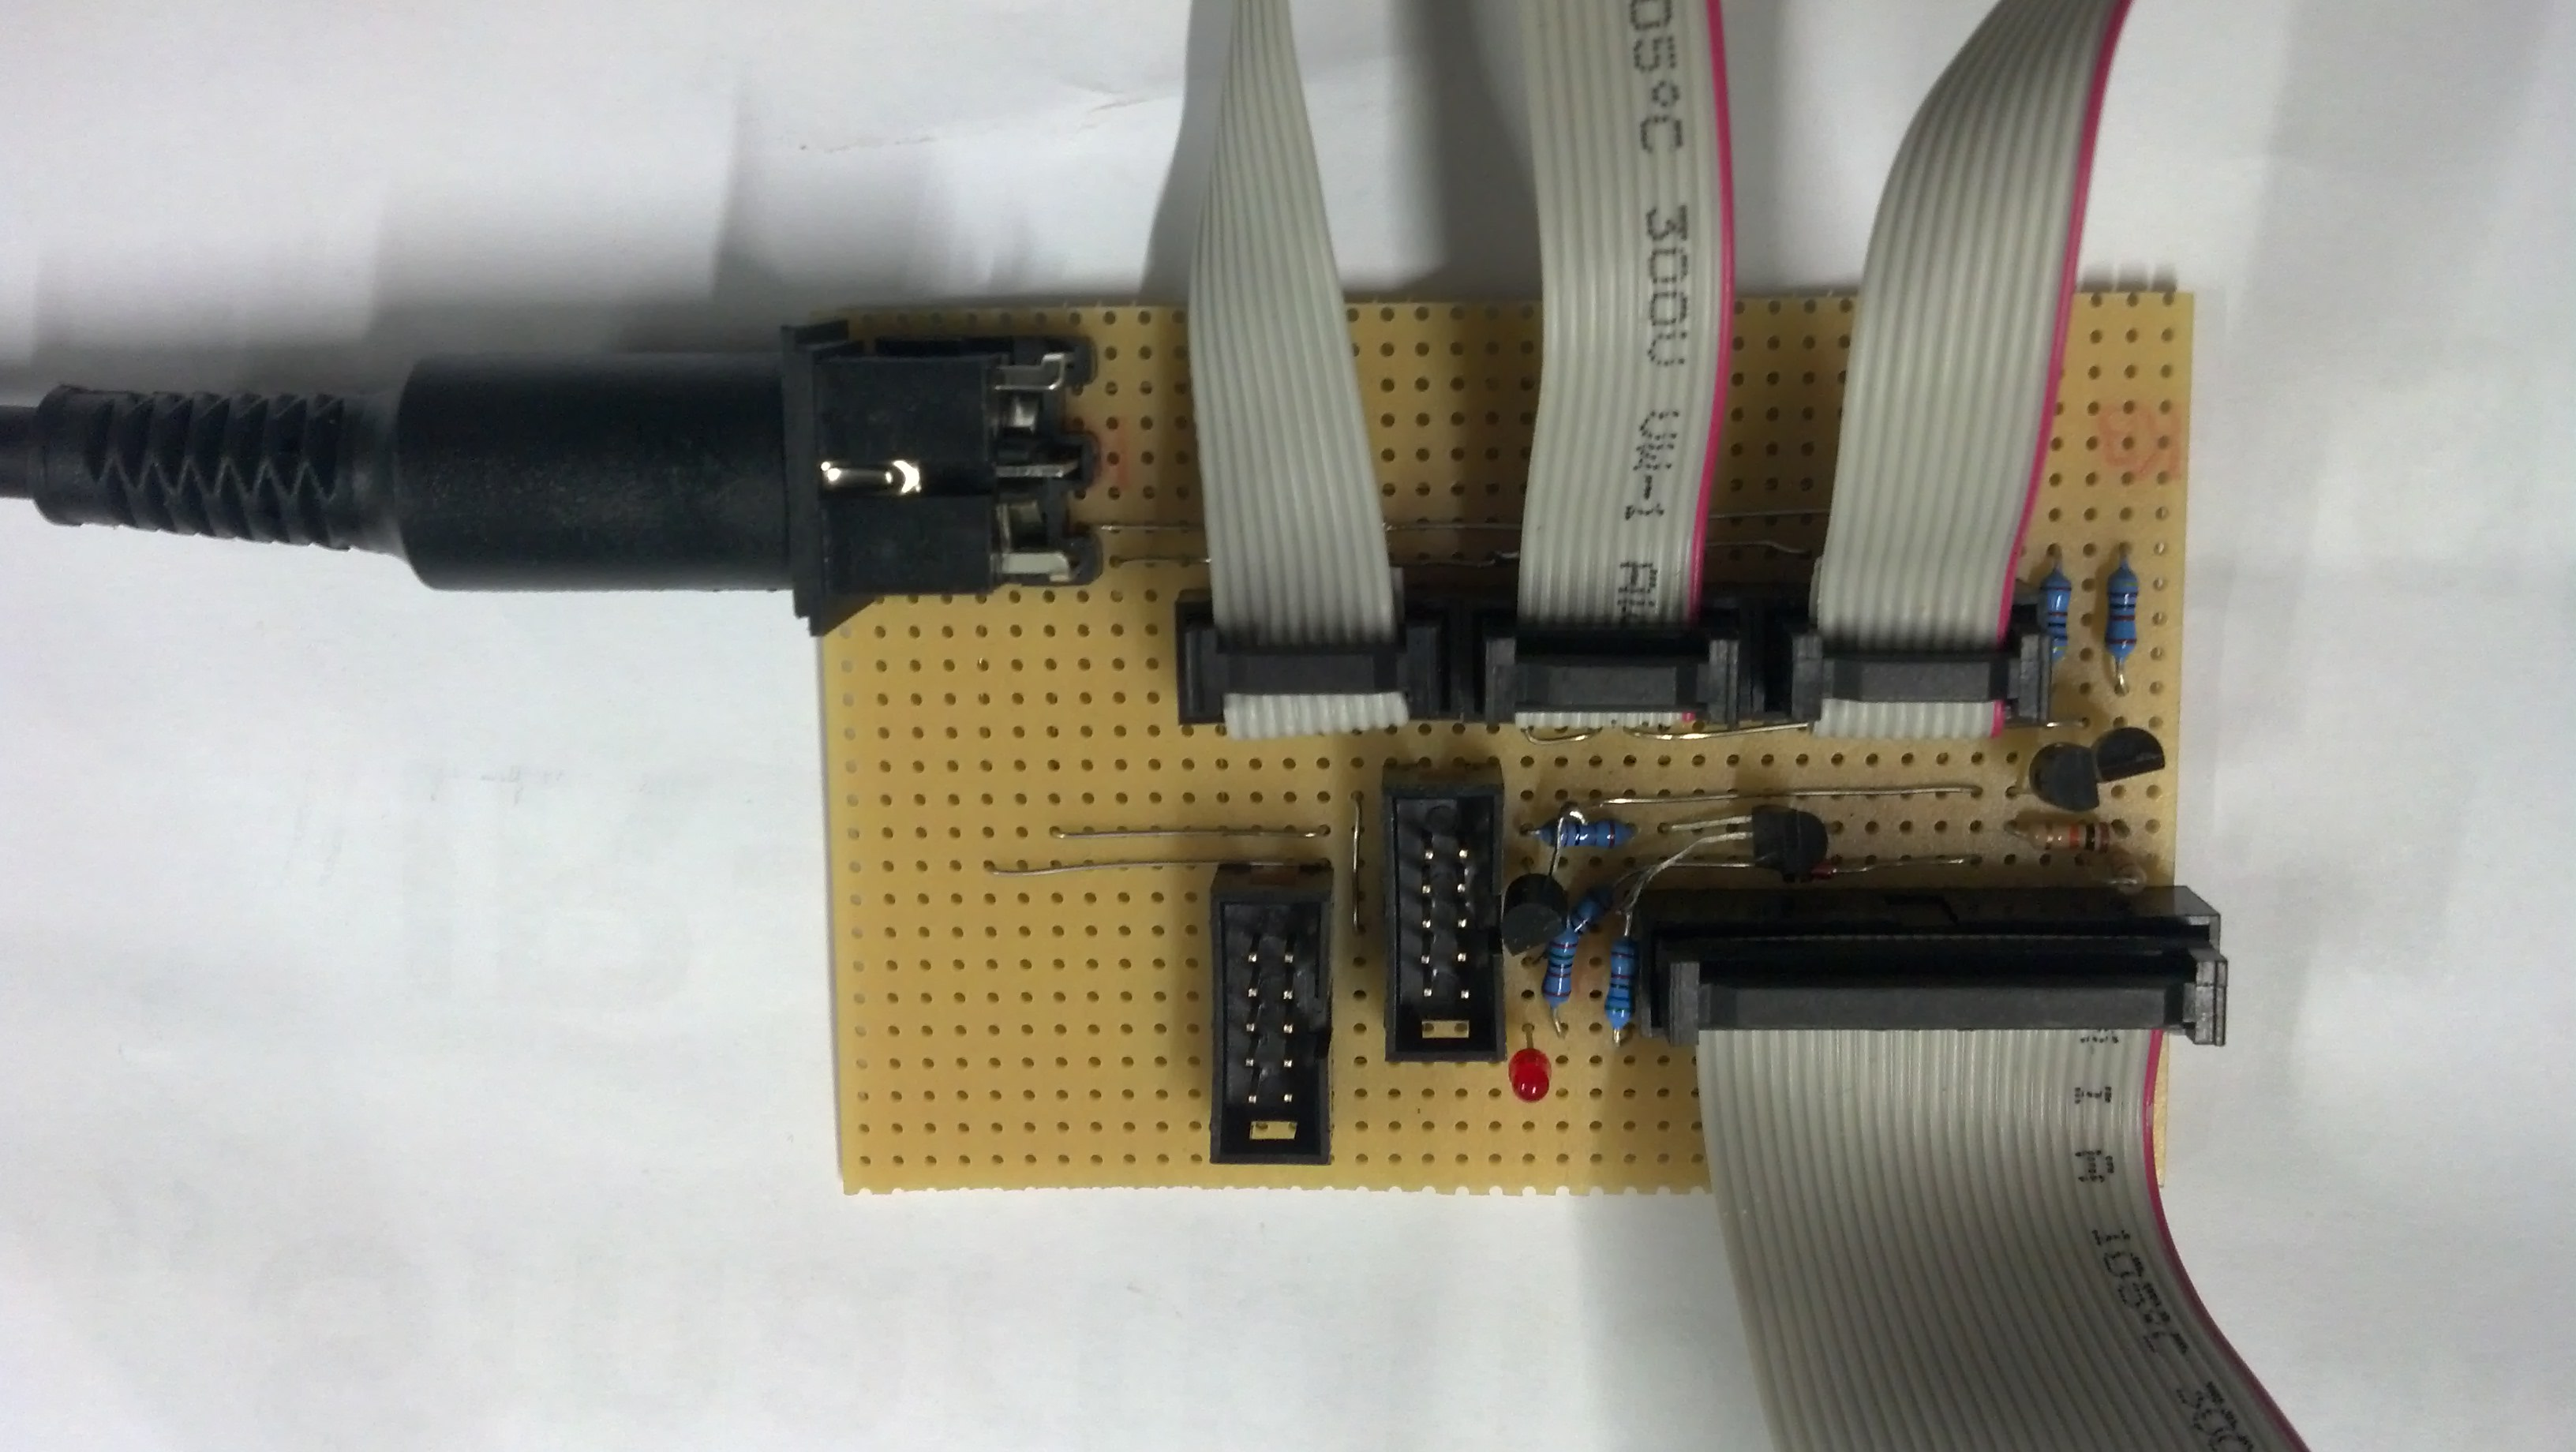
\includegraphics[width=(\textwidth), angle=0]{fotos/verteiler.jpg}
	\caption{Steckplätze der Verteiler-Platine} \label{p:2}
\end{figure}
Bei der Positionsbestimmung werden die Platinen in einem Dreieck angeordnet. Sie sind nummeriert und müssen gegen den Uhrzeigersinn geordnet sein. Positionen können innerhalb der eingespannten Fläche bestimmt werden, wobei eine Distanz von $15cm$ zu den Platinen eingehalten werden muss. \\
\begin{figure}[h]
	\centering
	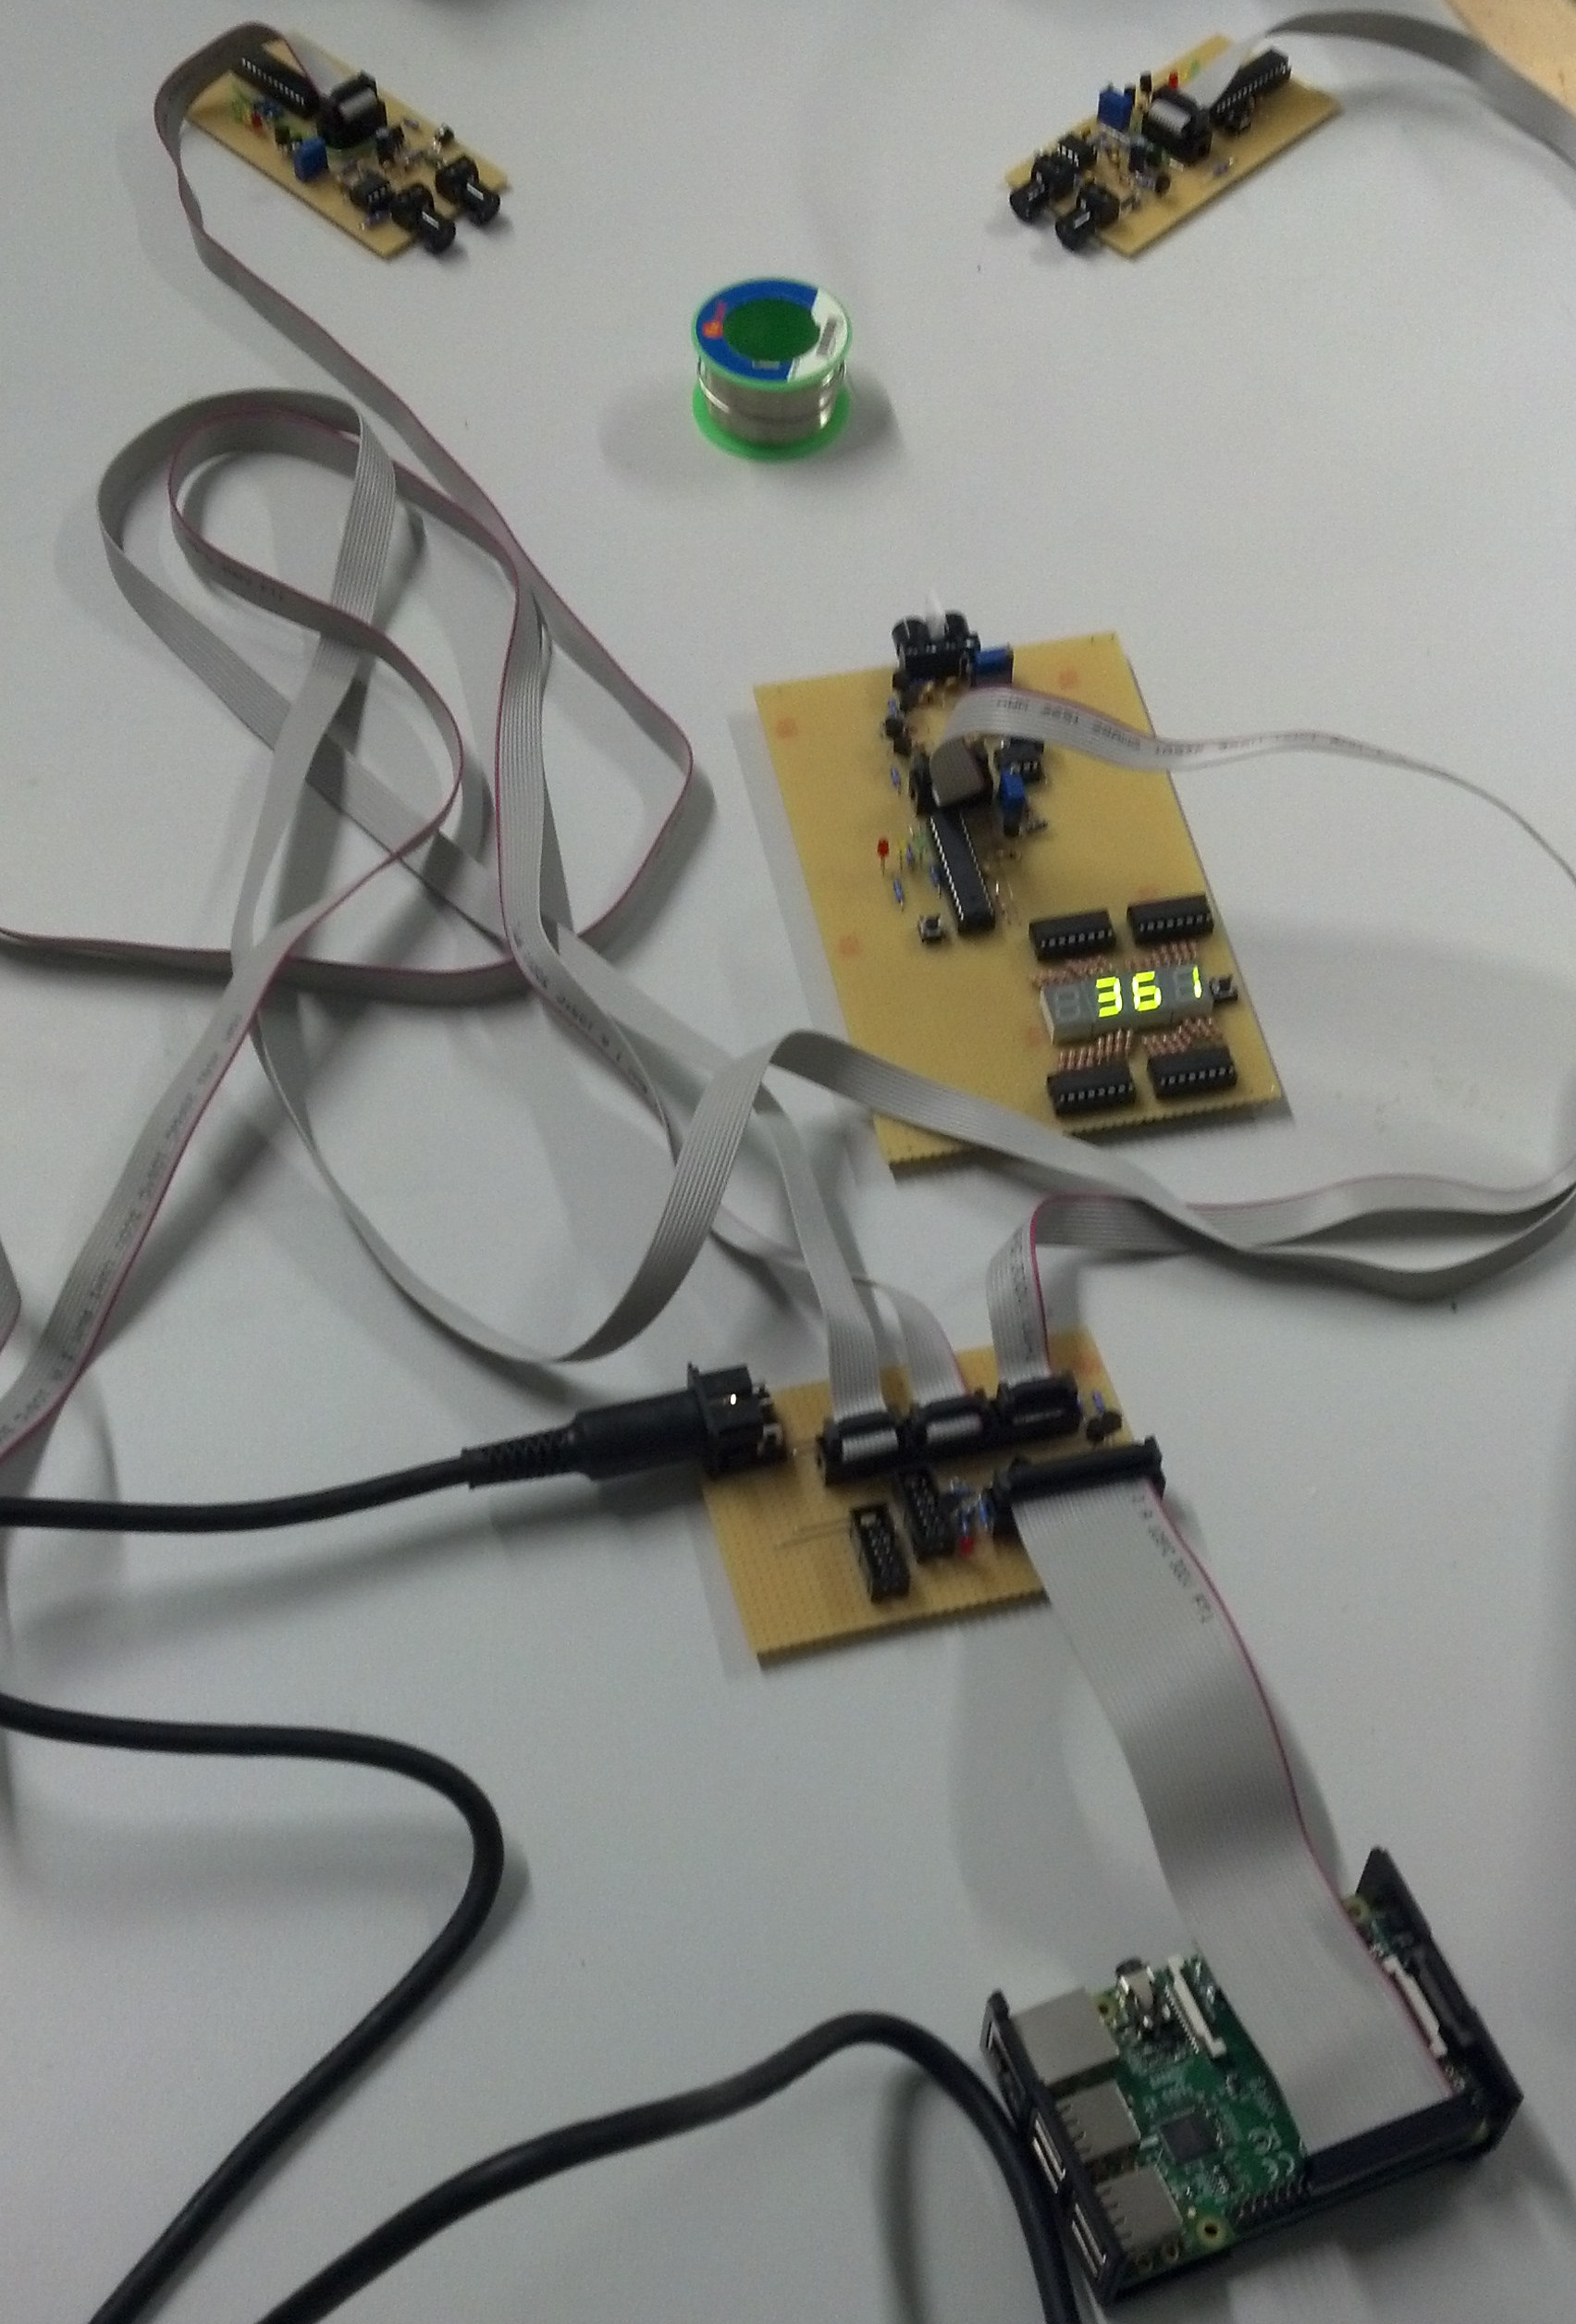
\includegraphics[width=(\textwidth), angle=0]{fotos/aufbau.jpg}
	\caption{Aufbau und Anordnung bei der Positionsbestimmung} \label{p:3}
\end{figure}
In der GUI können die Positionen der Sensoren bestimmt werden, damit eine exakte Positionsbestimmung relativ zu ihnen möglich ist.